\pgfdeclarelayer{background}
\pgfsetlayers{background,main}

\def\scale{0.62}

\tikzset{
  filled/.style={fill=circle area, draw=circle edge, thick}, outline/.style={draw=circle edge, thick}
  }

\setlength{\parskip}{5mm}

\tikzstyle{edge} = [draw, thick, -]

\tikzstyle{vertex}=[circle,fill=black!50,minimum size=10pt,inner sep=0pt]

\tikzstyle{selected edge} = [draw,line width=5pt,-,gray!50]
\tikzstyle{ignored edge} = [draw,line width=5pt,-,black!20]

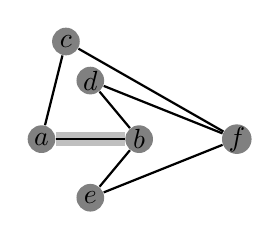
\begin{tikzpicture}[scale=\scale]
       \foreach \pos/\name in {{(0, 0)/a}, {(2, 0)/b}, {(0.5, 2)/c},  {(1, 1.2)/d}, {(1, -1.2)/e}, {(4,0)/f}} {
           \node[vertex] (\name) at \pos {$\name$};
%           \draw[outline] {\pos circle (1.5cm)} node {};
       }    

       \foreach \source/\sink in {a/c, a/b, c/f, b/d, b/e, e/f, d/f} {
           \path[edge] (\source) -- (\sink); 
       }
    \begin{pgfonlayer}{background}
      \foreach \source/ \dest in {a/b}
          \path[selected edge] (\source) -- (\dest);
    \end{pgfonlayer}
 
       
\end{tikzpicture}
